% ______________________________________________________________________________
%
%   2DV603 Software Engineering
%   Assignment 1 --- Requirements Engineering
%
%   Author:  Jonas Sjöberg
%            Linnaeus University
%            js224eh@student.lnu.se
%            github.com/jonasjberg
%            www.jonasjberg.com
%
%  License:  Creative Commons Attribution 4.0 International (CC BY 4.0)
%            <http://creativecommons.org/licenses/by/4.0/legalcode>
%            See LICENSE.md for additional licensing information.
% ______________________________________________________________________________


\section{Requirements Document}
% Task description from the assignment instructions
% \cite{2dv603:assignment1-instructions}:
% 
% \begin{quote}
%   Develop a full requirements definition for the above problem. Among the
%   techniques you should consider employing are the following: 1) take a look at
%   existing front-desk systems; 2) write scenarios; 3) derive use cases; 4)
%   perform use case analysis, to determine who the actors are and what tasks
%   they must perform; 5) narrow the problem statement, excluding features that
%   will not be needed in the first release.
% \end{quote}


\subsection{Scenarios}
These three scenarios are derived from the assignment instructions. \cite{2dv603:assignment1-instructions}

\subsubsection{Potential guest inquires about future patronage}\label{scenario1}
%
% clerk asks about:
%     * stay which nights?
%     * which type of room do they want?
%
% System must:
%
%   * verify if room(s) are available on those nights before allowing a reservation to be made
%   * verification procedure must take less than 2 seconds to complete.
%   * allow requests for specific rooms, controlled by the manage
%
\begin{itemize}
  \item A travelling salesman needs somewhere to stay for one night a couple of
    weeks from now.  This person contacts the hotel by phone to inquire about
    vacancy over a couple of days.  
    
  \item The hotel personnel answers any questions and uses the management
    system to find out if any rooms are available in the requested time frame.
    The hotel employee relays information about which rooms are available.

  \item After hearing about the rooms, the salesman asks about room sizes.

  \item The employee looks up relevant characteristics and attributes and
    relays the information.

  \item After brief contemplation, the salesman decides to make a reservation
    for one of the vacant rooms. 
\end{itemize}


\subsubsection{Guest checks in at the hotel}\label{scenario2}
% 
% * guest checks in
% 
%     * room is allocated until checkout
%     * must take in average less than 60 seconds to complete
% 
\begin{itemize}
  \item A travelling salesman arrives at the hotel after having sold nothing and has no patience for delays and pleasantries.
    He walks up to the hotel front desk and declares that he has made a reservation in advance and would like to check  in.
    
  \item The receptionist scrambles to find which room number the guest
    ostensibly has reserved. The receptionist asks the salesman for personal information used when making the reservation.

  \item The salesman provides personal information to the receptionist.
      
  \item The receptionist enters the information into the management system.
    After narrowing down the search results to a single number, the
    receptionist can retrieve the room key and proceed to guide the guest
    to his room.

  \item The salesman is provided with his room key and instructions on where
      the room is located.
\end{itemize}


\subsubsection{Guest cancels a reservation}\label{scenario3}
% 
% * guest wishes to cancel a reservation:
% 
%     * reservation can be canceled at any time but a percentage of the room
%       price may be charged if the cancelation is done too late
% 
\begin{itemize}
  \item A cat named Gibson wishes to cancel a reservation because of feline
      matters.  Gibson logs in to the hotel website using a identifier and
        access key that was provided to him when the room was first reserved.

  \item The web portal loads in under 2 seconds, which is probably considered good
        enough for a modern website. Gibson cries in cat but acknowledges that
        everything is really slow now and the hotel web portal is probably
        comparably ``performant''.

  \item After clicking on clearly visible ``cancel reservation'' link, a
      message informs Gibson about the cancellation fee, calculated from the
        room price and time delta from planned residence and cancellation.
      
  \item Gibson sighs in cat and clicks the ``I Agree'' link, which leads to a
      confirmation page with a summary of upayments that will be billed.
\end{itemize}




\subsection{Use Cases}

\begin{figure}[htbp]
  \centering
  \includegraphics[width=\linewidth]{include/uml-use-case-1.eps}
  \caption{UML Use Case Diagram for use case 1 -- Add a Book}
  \label{fig:uml-usecase1}
\end{figure}
%%% USECASES_START %%%

\subsubsection{Usecase --- Find Vacant Rooms}\label{usecase1}

\paragraph{Actors}

\begin{itemize}
\tightlist
\item
  Employee --- uses the system to gather information
\item
  Customer --- inquires about vacant rooms at a specific date
\end{itemize}

\paragraph{Goals}

\begin{itemize}
\tightlist
\item
  Find rooms that are vacant at a certain date
\item
  Respond to the customers inquiry
\end{itemize}

\paragraph{Preconditions}

\begin{itemize}
\tightlist
\item
  The system is ``live'' and reflects the actual state of the world
\item
  The employee is authorized to access information on room availability
\end{itemize}

\paragraph{Summary}

Demonstrates real-time use of the system to answer questions during
interaction with a customer.

\paragraph{Related}
This use case is extracted from Scenario~\ref{scenario1}.

\paragraph{Entry Conditions}

The employee wants to get information to provide to a customer during an
interaction.

\paragraph{Steps}

\begin{enumerate}
\def\labelenumi{\arabic{enumi}.}
\tightlist
\item
  Navigate to the room-search functionality
\item
  Enter the date of interest
\item
  Proceed to the results listing
\item
  Repeat steps 2--3 until all customer inquiries are resolved
\end{enumerate}

\paragraph{Exit Condition}

The employee can answer the customers requests through information
provided by the system.

\subsubsection{Use Case --- Find Vacant non-smoking Rooms}\label{usecase2}

\paragraph{Actors}

\begin{itemize}
\tightlist
\item
  Employee --- uses the system to gather information
\end{itemize}

\paragraph{Goals}

\begin{itemize}
\tightlist
\item
  Find rooms for non-smokers that are vacant at a certain date
\end{itemize}

\paragraph{Preconditions}

\begin{itemize}
\tightlist
\item
  The system is ``live'' and reflects the actual state of the world
\item
  At least one room is marked as a ``non-smoking'' room
\item
  The employee is authorized to access information on room availability
\end{itemize}

\paragraph{Summary}

Demonstrates room queries with a conditional.

\paragraph{Related}
This use case is extracted from Scenario~\ref{scenario1}.
It is also related to Usecase~\ref{usecase1}.

\paragraph{Entry Conditions}

The employee wants to find rooms for non-smokers that are vacant at a
certain date.

\paragraph{Steps}

\begin{enumerate}
\def\labelenumi{\arabic{enumi}.}
\tightlist
\item
  Navigate to the room-search functionality
\item
  Enter the date of interest
\item
  Enable filtering non-smoking rooms
\item
  Proceed to the results listing
\end{enumerate}

\paragraph{Exit Condition}

The employee has gathered information on whether there are vacant
non-smoking rooms at a given date.

\subsubsection{Use Case --- Reserve a Specific Room}\label{usecase3}

\paragraph{Actors}

\begin{itemize}
\tightlist
\item
  Manager --- uses the system to reserve a room
\item
  Customer --- wants to reserve a specific room
\end{itemize}

\paragraph{Goals}

\begin{itemize}
\tightlist
\item
  Make a reservation of a specific room
\end{itemize}

\paragraph{Preconditions}

\begin{itemize}
\tightlist
\item
  The system is ``live'' and reflects the actual state of the world
\item
  The manager can make reservations of specific rooms
\end{itemize}

\paragraph{Summary}

Involves a special kind of interaction \emph{that might require elevated
privileges}.

\paragraph{Entry Conditions}

The manager wants to meet a less frequent, specific request.

\paragraph{Steps}

\begin{enumerate}
\def\labelenumi{\arabic{enumi}.}
\tightlist
\item
  Navigate to the room-search functionality
\item
  Enter the room number of the requested room
\item
  See if it is currently vacant
\item
  If not:

  \begin{itemize}
  \tightlist
  \item
    Reserve the room
  \end{itemize}
\item
  If it is:

  \begin{itemize}
  \tightlist
  \item
    Attempt to exploit elevated privileges to invalidate the current
    vacancy
  \item
    Reserve the room
  \end{itemize}
\end{enumerate}

\paragraph{Exit Condition}

\begin{enumerate}
\def\labelenumi{\arabic{enumi}.}
\tightlist
\item
  The requested room is either already reserved and the manager can not
  meet the customer request.
\item
  The requested room is reserved.
\end{enumerate}

%%% USECASES_END %%%



\begin{figure}[htbp]
  \centering
  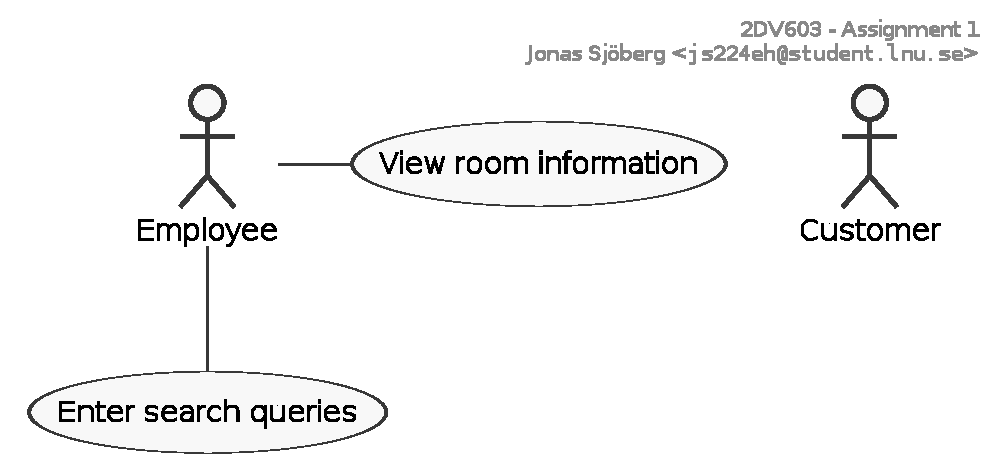
\includegraphics[width=\linewidth]{include/usecase1.eps}
  \caption{UML Use Case Diagram for Use Case 1 -- Get information on room}
  \label{fig:uml-usecase1}
\end{figure}

\begin{figure}[htbp]
  \centering
  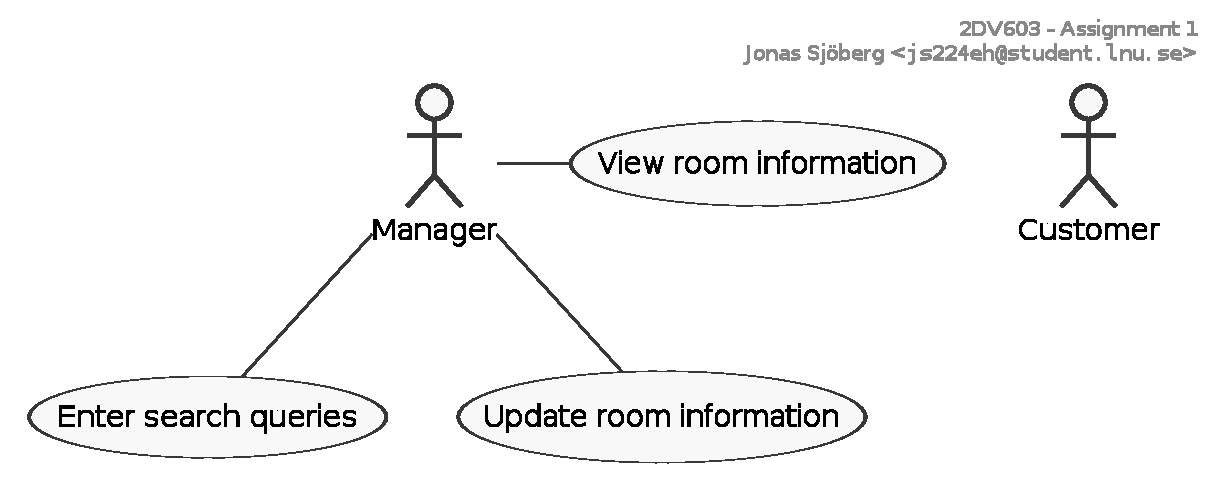
\includegraphics[width=\linewidth]{include/usecase2.eps}
  \caption{UML Use Case Diagram for Use Case 2 -- Get information on room and make a reservation}
  \label{fig:uml-usecase2}
\end{figure}


The UML use case diagram for Usecase~\ref{usecase1} and Usecase~\ref{usecase2} is shown in Figure~\ref{fig:uml-usecase1}.
The UML use case diagram for Usecase~\ref{usecase3} is shown in Figure~\ref{fig:uml-usecase2}.


\subsection{Use Case Analysis}
%
% TODO: Perform use case analysis to determine who the actors are and what tasks they must perform..
%


\subsection{Refined Problem Statement}
%
% TODO: Narrow the problem statement, excluding features that will not be needed in the first release ..
%
